\documentclass[12pt, a4paper]{article}
\usepackage{itmo}

\begin{document}
\kafedra{Кафедра вычислительной техники}
\title{Лабораторная работа №1}
\variant{Вариант 14}
\author{Пичугин~Н., гр.~3106}
%\authors{Пичугин~Н., гр.~3106 \\ Наумов~М., гр.~3106}
%\authorfem{Процаенко~О., гр.~3106}
\prepod{Косяков~М.~С.}
\maketitle

\tableofcontents
\newpage

\section*{Введение}
\addcontentsline{toc}{section}{Введение}

Если я предположу (Рис.~\ref{fig:sample1}), что между Землёй и Марсом 
вокруг Солнца по эллиптической орбите летает фарфоровый чайник, никто не 
сможет опровергнуть моё утверждение, особенно если я аккуратно добавлю, что 
чайник настолько мал, что не виден даже самыми мощнейшими 
телескопами~\cite{kubensky}. Но если бы я затем сказал, что если моё 
утверждение не может быть опровергнуто, то недопустимо человеческому 
разуму в нём сомневаться, мои слова следовало бы с полным на то основанием 
счесть бессмыслицей.
\par
Тем не менее, если существование такого чайника утверждалось бы в древних 
книгах~\cite{landin}, каждое воскресенье заучиваемых как святая истина, и 
насаждалось бы в умах школьников, то сомнение в его существовании стало бы 
признаком эксцентричности и привлекло бы к усомнившемуся внимание 
психиатра в наш просвещённый век, или же инквизитора в прошлом.

\begin{figure}[H]
    \centering
    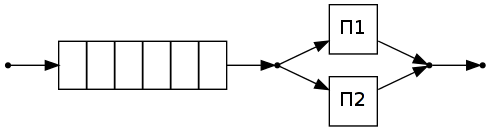
\includegraphics[width=0.8\textwidth]{sample1.png}
    \caption{Пример картинки}
    \label{fig:sample1}
\end{figure}

\section{Предлагаемые методы решения}
В каждой стране пропаганда контролируется государством и представляет 
собой то, что нравится государству. А что нравится государству, так это 
ваша готовность совершить убийство, когда вам прикажут.
\begin{description}  % opt: itemize, enumerate
    \item[Item 1:] Value 1
    \item[Item 2:] Value 2
    \item[Item 3:] Value 3
\end{description}

\section{Формулы}

$$\rho_{\square\textrm{опт}}=\sqrt{\frac{\sum\limits_{i=1}^{n} R_{i}}{\sum\limits_{i=1}^{n} R_{i}^{-1}}} = 1939,47 \approx 2000$$

$$b_T = \left\{ \begin{matrix} 0,2 \textrm{ мм при } \Delta R = \pm 20\% \\
0,3 \textrm{ мм при } \Delta R = \pm 10\%\end{matrix} \right. $$

\section{Исходный код}

\subsection{SumDigits.c}
\begin{verbatim}
#include <stdio.h>
#include <stdlib.h>

#define ERR_INCORRECT_BASE -1

int SumDigits(unsigned long long n, unsigned int base)
{
    if (base < 2)
        return ERR_INCORRECT_BASE;
    int sum = 0;
    for (; n; n /= base)
        sum += n % base;
    return sum;
}

int main(int argc, char **argv)
{
    printf("%d %d %d %d %d\n",
            SumDigits(1, 10),
            SumDigits(12345, 10),
            SumDigits(123045, 10),
            SumDigits(0xFE, 16),
            SumDigits(0xF0E, 16) );
    return EXIT_SUCCESS;
}
\end{verbatim}

\subsection{Результаты}
Результаты представлены в Табл.~\ref{table:results}.
\begin{table}[H]
\caption{Таблица результатов}
\centering
\begin{tabular}{| r | r |}
\hline
Входное значение & Результат \\ \hline
5 & 5 \\ \hline
56 & 11 \\ \hline
12345 & 15 \\ \hline
\end{tabular}
\label{table:results}
\end{table}


\subsection{Анализ}
Функция \texttt{SumDigits} принимает два аргумента: число и основание 
\emph{системы счисления}. Сначала проверяем последний на 
\textbf{некорректные} значения СС, после чего циклично получаем последнюю
цифру остающегося после целочисленного деления числа с помощью операции
получения остатка от деления и прибавляем ее к ответу. После этого 
возвращаем полученную сумму.

\makeatletter
\renewcommand{\@biblabel}[1]{#1.}
\makeatother
\bibliographystyle{utf8gost705u}
\bibliography{example}

\end{document}

